%%%%%%%%% BODY TEXT
%\vspace{-5mm}
\section{Introduction}

\begin{figure}[t]
\centering
   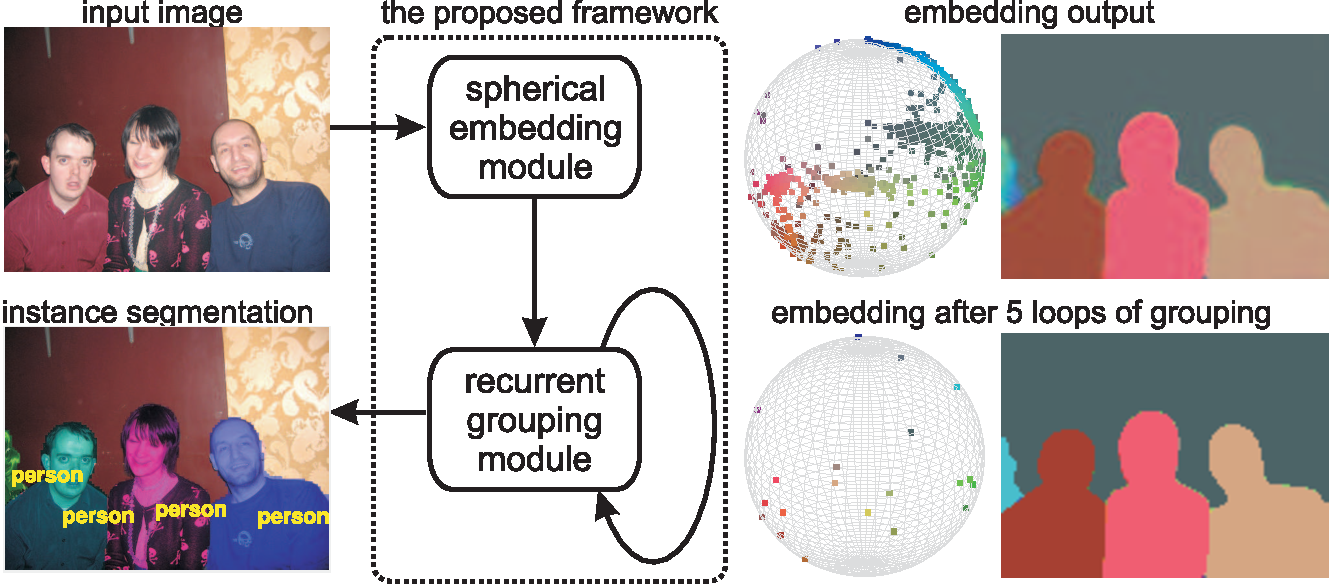
\includegraphics[width=0.995\linewidth]{splash_figure_ID12}
   \vspace{-3.5mm}
   \caption{
   \small Our framework embeds pixels into a hyper-sphere where
   recurrent mean-shift dynamics groups pixels
   into a variable number of object instances.  Here we visualize random
   projections of a 64-dim embeddings into 3-dimensions.
   }
   \vspace{-5.mm}
\label{fig:splash_figure}
\end{figure}

The successes of deep convolutional neural nets (CNNs) at image classification
has spawned a flurry of work in computer vision on adapting these models to
pixel-level image understanding tasks, such as boundary detection
\cite{arbelaez2011contour, xie2015holistically, maninis2017convolutional},
semantic segmentation \cite{long2015fully,chen2016deeplab,kong2017recurrent},
optical flow \cite{weinzaepfel2013deepflow, dosovitskiy2015flownet}, and pose
estimation \cite{wei2016cpm, cao2017realtime}.  The key ideas that have enabled
this adaption thus far are: (1) deconvolution schemes that allow for upsampling
coarse pooled feature maps to make detailed predictions at the spatial
resolution of individual pixels~\cite{xie2015holistically,ghiasi2016laplacian},
(2) skip connections and hyper-columns which concatenate representations across
multi-resolution feature maps~\cite{hariharan2015hypercolumns,chen2016deeplab},
(3) atrous convolution which allows efficient computation with large receptive
fields while maintaining spatial resolution~\cite{chen2016deeplab,
kong2017recurrent}, and (4) fully convolutional operation which handles
variable sized input images.

In contrast, there has been less innovation in the development of specialized
loss functions for training. Pixel-level labeling tasks fall into the category
of structured output prediction~\cite{bakir2007predicting}, where the model
outputs a structured object (e.g., a whole image parse) rather than a scalar or
categorical variable.  However, most CNN pixel-labeling architectures are
simply trained with loss functions that decompose into a simple (weighted) sum
of classification or regression losses over individual pixel labels.

The need to address the output space structure is more apparent when
considering problems where the set of output labels isn't fixed.  Our
motivating example is object instance segmentation, where the model generates a
collection of segments corresponding to object instances.  This problem
can't be treated as k-way classification since the number of objects isn't
known in advance.  Further, the loss should be invariant to permutations of
the instance labels within the same semantic category.
%(swapping identities of two instances doesn't change the output).




As a result, most recent successful approaches to instance segmentation have
adopted more heuristic approaches that first use an object detector to
enumerate candidate instances and then perform pixel-level segmentation of each
instance~\cite{liang2015proposal, dai2016instance, li2016fully,
liang2016reversible, arnab2017pixelwise}.  Alternately one can generate generic
proposal segments and then label each one with a semantic
detector~\cite{hariharan2014simultaneous, chen2015multi,
hariharan2015hypercolumns, dai2015convolutional, uhrig2016pixel, he2017mask}.
In either case the detection and segmentation steps can both be mapped to
standard binary classification losses.  While effective, these approaches are
somewhat unsatisfying since: (1) they rely on the object detector and
non-maximum suppression heuristics to accurately ``count'' the number of
instances, (2) they are difficult to train in an end-to-end manner since the
interface between instance segmentation and detection is non-differentiable,
and (3) they underperform in cluttered scenes as the assignment of pixels to
detections is carried out independently for each detection\footnote{This is
less a problem for object proposals that are jointly estimated by bottom-up
segmentation (e.g., MCG~\cite{pont2017multiscale} and COB
\cite{maninis2017convolutional}).  However, such generic proposal generation is
not informed by the top-down semantics.}.

Here we propose to directly tackle the instance grouping problem in a unified
architecture by training a model that labels pixels with unit-length vectors
that live in some fixed-dimension embedding space
(Fig.~\ref{fig:splash_figure}).  Unlike k-way classification where the target
vectors for each pixel are specified in advance (i.e., one-hot vectors at the
vertices of a k-1 dimensional simplex) we allow each instance to be labeled
with an arbitrary embedding vector on the sphere.  Our loss function simply
enforces the constraint that the embedding vectors used to label different
instances are far apart.  Since neither the number of labels, nor the target
label vectors are specified in advance, we can't use standard soft-max
thresholding to produce a discrete labeling.  Instead, we utilize a
variant of mean-shift clustering which can be viewed as a recurrent network
whose fixed point identifies a small, discrete set of instance label vectors
and concurrently labels each pixel with one of the vectors from this set.

This framework is largely agnostic to the underlying CNN architecture and can
be applied to a range of low, mid and high level visual tasks. Specifically,
we carry out experiments showing how this method can be used for boundary
detection, object proposal generation and semantic instance segmentation. Even
when a task can be modeled by a binary pixel classification loss (e.g.,
boundary detection) we find that the grouping loss guides the model towards
higher-quality feature representations that yield superior performance to
classification loss alone. The model really shines for instance segmentation,
where we demonstrate a substantial boost in object proposal generation
(improving the state-of-the-art average recall for 10 proposals per image from
0.56 to 0.77).  To summarize our contributions: (1) we introduce a simple,
easily interpreted end-to-end model for pixel-level instance labeling which is
widely applicable and highly effective, (2) we provide theoretical analysis
that offers guidelines on setting hyperparameters, and (3) benchmark results
show substantial improvements over existing approaches.


\section{Related Work}

Common approaches to instance segmentation first generate region proposals or
class-agnostic bounding boxes, segment the foreground objects within each
proposal and classify the objects in the bounding box~\cite{yang2012layered,
ladicky2010and, hariharan2014simultaneous, chen2015multi, dai2016instance,
liang2016reversible, he2017mask}.  \cite{li2016fully} introduce a fully
convolutional approach that includes bounding box proposal generation in
end-to-end training.  Recently, ``box-free''
methods~\cite{pinheiro2015learning, pinheiro2016learning, liang2015proposal,
hu2016fastmask} avoid some limitations of box proposals (e.g. for wiry or
articulated objects). They commonly use Faster RCNN~\cite{ren2015faster} to
produce ``centeredness'' score on each pixel and then predict binary instance
masks and class labels.  Other approaches have been explored for modeling joint
segmentation and instance labeling jointly in a combinatorial framework (e.g.,
\cite{kirillov2016instancecut}) but typically don't address end-to-end
learning.  Alternately, recurrent models that sequentially produce a list of
instances~\cite{romera2016recurrent,renend} offer another approach to address
variable sized output structures in a unified manner.

The most closely related to ours is the associative embedding work of
\cite{newell2016associative}, which demonstrated strong results for grouping
multi-person keypoints, and unpublished work from \cite{fathi2017semantic} on
metric learning for instance segmentation.  Our approach extends on these ideas
substantially by integrating recurrent mean-shift to directly generate the
final instances (rather than heuristic decoding or thresholding distance to
seed proposals). There is also an important and interesting connection to work
that has used embedding to separate instances where the embedding is directly
learned using a supervised regression loss rather than a pairwise associative
loss.  \cite{sironi2014multiscale} train a regressor that predicts the distance
to the contour centerline for boundary detection, while \cite{bai2016deep}
predict the distance transform of the instance masks which is then
post-processed with watershed transform to generate segments.
\cite{uhrig2016pixel} predict an embedding based on scene depth and direction
towards the instance center (like Hough voting).

Finally, we note that these ideas are related to work on using embedding for
solving pairwise clustering problems. For example, normalized cuts clusters
embedding vectors given by the eigenvectors of the normalized graph
Laplacian~\cite{shi2000normalized} and the spatial gradient of these embedding
vectors was used in~\cite{arbelaez2011contour} as a feature for boundary
detection. Rather than learning pairwise similarity from data and then
embedding prior to clustering (e.g., \cite{maire2016affinity}), we use a
pairwise loss but learn the embedding directly. Our recurrent mean-shift
grouping is reminiscent of other efforts that use unrolled implementations of
iterative algorithms such as CRF inference~\cite{zheng2015conditional} or
bilateral filtering~\cite{jampani2016learning, gadde2015superpixel}. Unlike
general RNNs~\cite{bengio1994learning, pascanu2013difficulty} which are often
difficult to train, our recurrent model has fixed parameters that assure
interpretable convergent dynamics and meaningful gradients during learning.

%\subsubsection*{Mean Shift}
%\cite{kobayashi2010mises} introduces a normalized mean shift to deal with Von Mises-Fisher distribution.
%\cite{carreira2008generalised} discusses the $\bf P$ for mean shift and compares the speed, relationship to spectral clustering.
%\cite{carreira2006fast} introduces a stopping criterion and proves the convergence of cubic order with Gaussian clusters.
%\cite{solomon2014general, tomasi1998bilateral} introduces a way to encode spatial term to the intensity term.
%
%\subsection*{Maximum Margin}
%Weinberger \etal propose a loss function as below~\cite{weinberger2009distance}:
%\begin{equation}
%\begin{split}
%l = &\sum_{i,j} \eta_{ij} \Vert {\bf L} (\x_i-\x_j)\Vert_2^2 + \\
%    &c\sum_{i,j,l}\eta_{ij}(1-y_{il})[1+\Vert{\bf L} (\x_i-\x_j)\Vert_2^2-\Vert{\bf L} (\x_i-\x_l)\Vert_2^2]_{+}
%\end{split}
%\end{equation}
%
%
%Kong \etal propose a pairwise rank loss as below~\cite{kong2016photo}:
%\begin{equation}
%\begin{split}
%l = &\sum_{i,j} [\alpha-\delta(y_i>y_j) (\x_i-\x_j)]_{+}
%\end{split}
%\end{equation}
%
%
%\subsection*{Random Pixel Sampling}
%PixelNet~\cite{bansal2016pixelnet},
%Sampling matters in deep embedding learning~\cite{wu2017sampling}.
%
%
%
%\subsection*{Boundary Detection}
%HED~\cite{xie2015holistically},
%CEDN~\cite{yang2016object},
%LEP~\cite{najman1996geodesic},
%UCM~\cite{arbelaez2011contour},
%ISCRA~\cite{ren2013image},
%NCuts~\cite{shi2000normalized},
%EGB~\cite{felzenszwalb2004efficient},
%and MShift~\cite{comaniciu2002mean}.
%





